\documentclass{report}

%%%%%%%%%%%%%%%%%%%%%%%%%%%%%%%%%
% PACKAGE IMPORTS
%%%%%%%%%%%%%%%%%%%%%%%%%%%%%%%%%


\usepackage[tmargin=2cm,rmargin=1in,lmargin=1in,margin=0.85in,bmargin=2cm,footskip=.2in]{geometry}
\usepackage{amsmath,amsfonts,amsthm,amssymb,mathtools}
\usepackage[varbb]{newpxmath}
\usepackage{xfrac}
\usepackage[makeroom]{cancel}
\usepackage{mathtools}
\usepackage{bookmark}
\usepackage{enumitem}
\usepackage{hyperref,theoremref}
\hypersetup{
	pdftitle={Assignment},
	colorlinks=true, linkcolor=doc!90,
	bookmarksnumbered=true,
	bookmarksopen=true
}
\usepackage[most,many,breakable]{tcolorbox}
\usepackage{xcolor}
\usepackage{varwidth}
\usepackage{varwidth}
\usepackage{etoolbox}
\usepackage{caption}
\usepackage{subcaption}
%\usepackage{authblk}
\usepackage{nameref}
\usepackage{multicol,array}
\usepackage{tikz-cd}
\usepackage[ruled,vlined,linesnumbered]{algorithm2e}
\usepackage{comment} % enables the use of multi-line comments (\ifx \fi) 
\usepackage{import}
\usepackage{xifthen}
\usepackage{pdfpages}
\usepackage{transparent}
\usepackage{graphicx}
\usepackage[utf8]{inputenc}
\newcommand\mycommfont[1]{\footnotesize\ttfamily\textcolor{blue}{#1}}
\SetCommentSty{mycommfont}
\newcommand{\incfig}[1]{%
    \def\svgwidth{\columnwidth}
    \import{./figures/}{#1.pdf_tex}
}

\usepackage{tikzsymbols}
\renewcommand\qedsymbol{$\Laughey$}


%\usepackage{import}
%\usepackage{xifthen}
%\usepackage{pdfpages}
%\usepackage{transparent}


%%%%%%%%%%%%%%%%%%%%%%%%%%%%%%
% SELF MADE COLORS
%%%%%%%%%%%%%%%%%%%%%%%%%%%%%%



\definecolor{myg}{RGB}{56, 140, 70}
\definecolor{myb}{RGB}{45, 111, 177}
\definecolor{myr}{RGB}{199, 68, 64}
\definecolor{mytheorembg}{HTML}{F2F2F9}
\definecolor{mytheoremfr}{HTML}{00007B}
\definecolor{mylenmabg}{HTML}{FFFAF8}
\definecolor{mylenmafr}{HTML}{983b0f}
\definecolor{mypropbg}{HTML}{f2fbfc}
\definecolor{mypropfr}{HTML}{191971}
\definecolor{myexamplebg}{HTML}{F2FBF8}
\definecolor{myexamplefr}{HTML}{88D6D1}
\definecolor{myexampleti}{HTML}{2A7F7F}
\definecolor{mydefinitbg}{HTML}{E5E5FF}
\definecolor{mydefinitfr}{HTML}{3F3FA3}
\definecolor{notesgreen}{RGB}{0,162,0}
\definecolor{myp}{RGB}{197, 92, 212}
\definecolor{mygr}{HTML}{2C3338}
\definecolor{myred}{RGB}{127,0,0}
\definecolor{myyellow}{RGB}{169,121,69}
\definecolor{myexercisebg}{HTML}{F2FBF8}
\definecolor{myexercisefg}{HTML}{88D6D1}


%%%%%%%%%%%%%%%%%%%%%%%%%%%%
% TCOLORBOX SETUPS
%%%%%%%%%%%%%%%%%%%%%%%%%%%%

\setlength{\parindent}{1cm}
%================================
% THEOREM BOX
%================================

\tcbuselibrary{theorems,skins,hooks}
\newtcbtheorem[number within=section]{Theorem}{Theorem}
{%
	enhanced,
	breakable,
	colback = mytheorembg,
	frame hidden,
	boxrule = 0sp,
	borderline west = {2pt}{0pt}{mytheoremfr},
	sharp corners,
	detach title,
	before upper = \tcbtitle\par\smallskip,
	coltitle = mytheoremfr,
	fonttitle = \bfseries\sffamily,
	description font = \mdseries,
	separator sign none,
	segmentation style={solid, mytheoremfr},
}
{th}

\tcbuselibrary{theorems,skins,hooks}
\newtcbtheorem[number within=chapter]{theorem}{Theorem}
{%
	enhanced,
	breakable,
	colback = mytheorembg,
	frame hidden,
	boxrule = 0sp,
	borderline west = {2pt}{0pt}{mytheoremfr},
	sharp corners,
	detach title,
	before upper = \tcbtitle\par\smallskip,
	coltitle = mytheoremfr,
	fonttitle = \bfseries\sffamily,
	description font = \mdseries,
	separator sign none,
	segmentation style={solid, mytheoremfr},
}
{th}


\tcbuselibrary{theorems,skins,hooks}
\newtcolorbox{Theoremcon}
{%
	enhanced
	,breakable
	,colback = mytheorembg
	,frame hidden
	,boxrule = 0sp
	,borderline west = {2pt}{0pt}{mytheoremfr}
	,sharp corners
	,description font = \mdseries
	,separator sign none
}

%================================
% Corollery
%================================
\tcbuselibrary{theorems,skins,hooks}
\newtcbtheorem[number within=section]{Corollary}{Corollary}
{%
	enhanced
	,breakable
	,colback = myp!10
	,frame hidden
	,boxrule = 0sp
	,borderline west = {2pt}{0pt}{myp!85!black}
	,sharp corners
	,detach title
	,before upper = \tcbtitle\par\smallskip
	,coltitle = myp!85!black
	,fonttitle = \bfseries\sffamily
	,description font = \mdseries
	,separator sign none
	,segmentation style={solid, myp!85!black}
}
{th}
\tcbuselibrary{theorems,skins,hooks}
\newtcbtheorem[number within=chapter]{corollary}{Corollary}
{%
	enhanced
	,breakable
	,colback = myp!10
	,frame hidden
	,boxrule = 0sp
	,borderline west = {2pt}{0pt}{myp!85!black}
	,sharp corners
	,detach title
	,before upper = \tcbtitle\par\smallskip
	,coltitle = myp!85!black
	,fonttitle = \bfseries\sffamily
	,description font = \mdseries
	,separator sign none
	,segmentation style={solid, myp!85!black}
}
{th}


%================================
% LENMA
%================================

\tcbuselibrary{theorems,skins,hooks}
\newtcbtheorem[number within=section]{Lenma}{Lenma}
{%
	enhanced,
	breakable,
	colback = mylenmabg,
	frame hidden,
	boxrule = 0sp,
	borderline west = {2pt}{0pt}{mylenmafr},
	sharp corners,
	detach title,
	before upper = \tcbtitle\par\smallskip,
	coltitle = mylenmafr,
	fonttitle = \bfseries\sffamily,
	description font = \mdseries,
	separator sign none,
	segmentation style={solid, mylenmafr},
}
{th}

\tcbuselibrary{theorems,skins,hooks}
\newtcbtheorem[number within=chapter]{lenma}{Lenma}
{%
	enhanced,
	breakable,
	colback = mylenmabg,
	frame hidden,
	boxrule = 0sp,
	borderline west = {2pt}{0pt}{mylenmafr},
	sharp corners,
	detach title,
	before upper = \tcbtitle\par\smallskip,
	coltitle = mylenmafr,
	fonttitle = \bfseries\sffamily,
	description font = \mdseries,
	separator sign none,
	segmentation style={solid, mylenmafr},
}
{th}


%================================
% PROPOSITION
%================================

\tcbuselibrary{theorems,skins,hooks}
\newtcbtheorem[number within=section]{Prop}{Proposition}
{%
	enhanced,
	breakable,
	colback = mypropbg,
	frame hidden,
	boxrule = 0sp,
	borderline west = {2pt}{0pt}{mypropfr},
	sharp corners,
	detach title,
	before upper = \tcbtitle\par\smallskip,
	coltitle = mypropfr,
	fonttitle = \bfseries\sffamily,
	description font = \mdseries,
	separator sign none,
	segmentation style={solid, mypropfr},
}
{th}

\tcbuselibrary{theorems,skins,hooks}
\newtcbtheorem[number within=chapter]{prop}{Proposition}
{%
	enhanced,
	breakable,
	colback = mypropbg,
	frame hidden,
	boxrule = 0sp,
	borderline west = {2pt}{0pt}{mypropfr},
	sharp corners,
	detach title,
	before upper = \tcbtitle\par\smallskip,
	coltitle = mypropfr,
	fonttitle = \bfseries\sffamily,
	description font = \mdseries,
	separator sign none,
	segmentation style={solid, mypropfr},
}
{th}


%================================
% CLAIM
%================================

\tcbuselibrary{theorems,skins,hooks}
\newtcbtheorem[number within=section]{claim}{Claim}
{%
	enhanced
	,breakable
	,colback = myg!10
	,frame hidden
	,boxrule = 0sp
	,borderline west = {2pt}{0pt}{myg}
	,sharp corners
	,detach title
	,before upper = \tcbtitle\par\smallskip
	,coltitle = myg!85!black
	,fonttitle = \bfseries\sffamily
	,description font = \mdseries
	,separator sign none
	,segmentation style={solid, myg!85!black}
}
{th}



%================================
% Exercise
%================================

\tcbuselibrary{theorems,skins,hooks}
\newtcbtheorem[number within=section]{Exercise}{Exercise}
{%
	enhanced,
	breakable,
	colback = myexercisebg,
	frame hidden,
	boxrule = 0sp,
	borderline west = {2pt}{0pt}{myexercisefg},
	sharp corners,
	detach title,
	before upper = \tcbtitle\par\smallskip,
	coltitle = myexercisefg,
	fonttitle = \bfseries\sffamily,
	description font = \mdseries,
	separator sign none,
	segmentation style={solid, myexercisefg},
}
{th}

\tcbuselibrary{theorems,skins,hooks}
\newtcbtheorem[number within=chapter]{exercise}{Exercise}
{%
	enhanced,
	breakable,
	colback = myexercisebg,
	frame hidden,
	boxrule = 0sp,
	borderline west = {2pt}{0pt}{myexercisefg},
	sharp corners,
	detach title,
	before upper = \tcbtitle\par\smallskip,
	coltitle = myexercisefg,
	fonttitle = \bfseries\sffamily,
	description font = \mdseries,
	separator sign none,
	segmentation style={solid, myexercisefg},
}
{th}

%================================
% EXAMPLE BOX
%================================

\newtcbtheorem[number within=section]{Example}{Example}
{%
	colback = myexamplebg
	,breakable
	,colframe = myexamplefr
	,coltitle = myexampleti
	,boxrule = 1pt
	,sharp corners
	,detach title
	,before upper=\tcbtitle\par\smallskip
	,fonttitle = \bfseries
	,description font = \mdseries
	,separator sign none
	,description delimiters parenthesis
}
{ex}

\newtcbtheorem[number within=chapter]{example}{Example}
{%
	colback = myexamplebg
	,breakable
	,colframe = myexamplefr
	,coltitle = myexampleti
	,boxrule = 1pt
	,sharp corners
	,detach title
	,before upper=\tcbtitle\par\smallskip
	,fonttitle = \bfseries
	,description font = \mdseries
	,separator sign none
	,description delimiters parenthesis
}
{ex}

%================================
% DEFINITION BOX
%================================

\newtcbtheorem[number within=section]{Definition}{Definition}{enhanced,
	before skip=2mm,after skip=2mm, colback=red!5,colframe=red!80!black,boxrule=0.5mm,
	attach boxed title to top left={xshift=1cm,yshift*=1mm-\tcboxedtitleheight}, varwidth boxed title*=-3cm,
	boxed title style={frame code={
					\path[fill=tcbcolback]
					([yshift=-1mm,xshift=-1mm]frame.north west)
					arc[start angle=0,end angle=180,radius=1mm]
					([yshift=-1mm,xshift=1mm]frame.north east)
					arc[start angle=180,end angle=0,radius=1mm];
					\path[left color=tcbcolback!60!black,right color=tcbcolback!60!black,
						middle color=tcbcolback!80!black]
					([xshift=-2mm]frame.north west) -- ([xshift=2mm]frame.north east)
					[rounded corners=1mm]-- ([xshift=1mm,yshift=-1mm]frame.north east)
					-- (frame.south east) -- (frame.south west)
					-- ([xshift=-1mm,yshift=-1mm]frame.north west)
					[sharp corners]-- cycle;
				},interior engine=empty,
		},
	fonttitle=\bfseries,
	title={#2},#1}{def}
\newtcbtheorem[number within=chapter]{definition}{Definition}{enhanced,
	before skip=2mm,after skip=2mm, colback=red!5,colframe=red!80!black,boxrule=0.5mm,
	attach boxed title to top left={xshift=1cm,yshift*=1mm-\tcboxedtitleheight}, varwidth boxed title*=-3cm,
	boxed title style={frame code={
					\path[fill=tcbcolback]
					([yshift=-1mm,xshift=-1mm]frame.north west)
					arc[start angle=0,end angle=180,radius=1mm]
					([yshift=-1mm,xshift=1mm]frame.north east)
					arc[start angle=180,end angle=0,radius=1mm];
					\path[left color=tcbcolback!60!black,right color=tcbcolback!60!black,
						middle color=tcbcolback!80!black]
					([xshift=-2mm]frame.north west) -- ([xshift=2mm]frame.north east)
					[rounded corners=1mm]-- ([xshift=1mm,yshift=-1mm]frame.north east)
					-- (frame.south east) -- (frame.south west)
					-- ([xshift=-1mm,yshift=-1mm]frame.north west)
					[sharp corners]-- cycle;
				},interior engine=empty,
		},
	fonttitle=\bfseries,
	title={#2},#1}{def}



%================================
% Solution BOX
%================================

\makeatletter
\newtcbtheorem{question}{Question}{enhanced,
	breakable,
	colback=white,
	colframe=myb!80!black,
	attach boxed title to top left={yshift*=-\tcboxedtitleheight},
	fonttitle=\bfseries,
	title={#2},
	boxed title size=title,
	boxed title style={%
			sharp corners,
			rounded corners=northwest,
			colback=tcbcolframe,
			boxrule=0pt,
		},
	underlay boxed title={%
			\path[fill=tcbcolframe] (title.south west)--(title.south east)
			to[out=0, in=180] ([xshift=5mm]title.east)--
			(title.center-|frame.east)
			[rounded corners=\kvtcb@arc] |-
			(frame.north) -| cycle;
		},
	#1
}{def}
\makeatother

%================================
% SOLUTION BOX
%================================

\makeatletter
\newtcolorbox{solution}{enhanced,
	breakable,
	colback=white,
	colframe=myg!80!black,
	attach boxed title to top left={yshift*=-\tcboxedtitleheight},
	title=Solution,
	boxed title size=title,
	boxed title style={%
			sharp corners,
			rounded corners=northwest,
			colback=tcbcolframe,
			boxrule=0pt,
		},
	underlay boxed title={%
			\path[fill=tcbcolframe] (title.south west)--(title.south east)
			to[out=0, in=180] ([xshift=5mm]title.east)--
			(title.center-|frame.east)
			[rounded corners=\kvtcb@arc] |-
			(frame.north) -| cycle;
		},
}
\makeatother

%================================
% Question BOX
%================================

\makeatletter
\newtcbtheorem{qstion}{Question}{enhanced,
	breakable,
	colback=white,
	colframe=mygr,
	attach boxed title to top left={yshift*=-\tcboxedtitleheight},
	fonttitle=\bfseries,
	title={#2},
	boxed title size=title,
	boxed title style={%
			sharp corners,
			rounded corners=northwest,
			colback=tcbcolframe,
			boxrule=0pt,
		},
	underlay boxed title={%
			\path[fill=tcbcolframe] (title.south west)--(title.south east)
			to[out=0, in=180] ([xshift=5mm]title.east)--
			(title.center-|frame.east)
			[rounded corners=\kvtcb@arc] |-
			(frame.north) -| cycle;
		},
	#1
}{def}
\makeatother

\newtcbtheorem[number within=chapter]{wconc}{Wrong Concept}{
	breakable,
	enhanced,
	colback=white,
	colframe=myr,
	arc=0pt,
	outer arc=0pt,
	fonttitle=\bfseries\sffamily\large,
	colbacktitle=myr,
	attach boxed title to top left={},
	boxed title style={
			enhanced,
			skin=enhancedfirst jigsaw,
			arc=3pt,
			bottom=0pt,
			interior style={fill=myr}
		},
	#1
}{def}



%================================
% NOTE BOX
%================================

\usetikzlibrary{arrows,calc,shadows.blur}
\tcbuselibrary{skins}
\newtcolorbox{note}[1][]{%
	enhanced jigsaw,
	colback=gray!20!white,%
	colframe=gray!80!black,
	size=small,
	boxrule=1pt,
	title=\textbf{Note:-},
	halign title=flush center,
	coltitle=black,
	breakable,
	drop shadow=black!50!white,
	attach boxed title to top left={xshift=1cm,yshift=-\tcboxedtitleheight/2,yshifttext=-\tcboxedtitleheight/2},
	minipage boxed title=1.5cm,
	boxed title style={%
			colback=white,
			size=fbox,
			boxrule=1pt,
			boxsep=2pt,
			underlay={%
					\coordinate (dotA) at ($(interior.west) + (-0.5pt,0)$);
					\coordinate (dotB) at ($(interior.east) + (0.5pt,0)$);
					\begin{scope}
						\clip (interior.north west) rectangle ([xshift=3ex]interior.east);
						\filldraw [white, blur shadow={shadow opacity=60, shadow yshift=-.75ex}, rounded corners=2pt] (interior.north west) rectangle (interior.south east);
					\end{scope}
					\begin{scope}[gray!80!black]
						\fill (dotA) circle (2pt);
						\fill (dotB) circle (2pt);
					\end{scope}
				},
		},
	#1,
}

%%%%%%%%%%%%%%%%%%%%%%%%%%%%%%
% SELF MADE COMMANDS
%%%%%%%%%%%%%%%%%%%%%%%%%%%%%%


\newcommand{\thm}[2]{\begin{Theorem}{#1}{}#2\end{Theorem}}
\newcommand{\cor}[2]{\begin{Corollary}{#1}{}#2\end{Corollary}}
\newcommand{\mlenma}[2]{\begin{Lenma}{#1}{}#2\end{Lenma}}
\newcommand{\mprop}[2]{\begin{Prop}{#1}{}#2\end{Prop}}
\newcommand{\clm}[3]{\begin{claim}{#1}{#2}#3\end{claim}}
\newcommand{\wc}[2]{\begin{wconc}{#1}{}\setlength{\parindent}{1cm}#2\end{wconc}}
\newcommand{\thmcon}[1]{\begin{Theoremcon}{#1}\end{Theoremcon}}
\newcommand{\ex}[2]{\begin{Example}{#1}{}#2\end{Example}}
\newcommand{\dfn}[2]{\begin{Definition}[colbacktitle=red!75!black]{#1}{}#2\end{Definition}}
\newcommand{\dfnc}[2]{\begin{definition}[colbacktitle=red!75!black]{#1}{}#2\end{definition}}
\newcommand{\qs}[2]{\begin{question}{#1}{}#2\end{question}}
\newcommand{\pf}[2]{\begin{myproof}[#1]#2\end{myproof}}
\newcommand{\nt}[1]{\begin{note}#1\end{note}}

\newcommand*\circled[1]{\tikz[baseline=(char.base)]{
		\node[shape=circle,draw,inner sep=1pt] (char) {#1};}}
\newcommand\getcurrentref[1]{%
	\ifnumequal{\value{#1}}{0}
	{??}
	{\the\value{#1}}%
}
\newcommand{\getCurrentSectionNumber}{\getcurrentref{section}}
\newenvironment{myproof}[1][\proofname]{%
	\proof[\bfseries #1: ]%
}{\endproof}

\newcommand{\mclm}[2]{\begin{myclaim}[#1]#2\end{myclaim}}
\newenvironment{myclaim}[1][\claimname]{\proof[\bfseries #1: ]}{}

\newcounter{mylabelcounter}

\makeatletter
\newcommand{\setword}[2]{%
	\phantomsection
	#1\def\@currentlabel{\unexpanded{#1}}\label{#2}%
}
\makeatother




\tikzset{
	symbol/.style={
			draw=none,
			every to/.append style={
					edge node={node [sloped, allow upside down, auto=false]{$#1$}}}
		}
}


% deliminators
\DeclarePairedDelimiter{\abs}{\lvert}{\rvert}
\DeclarePairedDelimiter{\norm}{\lVert}{\rVert}

\DeclarePairedDelimiter{\ceil}{\lceil}{\rceil}
\DeclarePairedDelimiter{\floor}{\lfloor}{\rfloor}
\DeclarePairedDelimiter{\round}{\lfloor}{\rceil}

\newsavebox\diffdbox
\newcommand{\slantedromand}{{\mathpalette\makesl{d}}}
\newcommand{\makesl}[2]{%
\begingroup
\sbox{\diffdbox}{$\mathsurround=0pt#1\mathrm{#2}$}%
\pdfsave
\pdfsetmatrix{1 0 0.2 1}%
\rlap{\usebox{\diffdbox}}%
\pdfrestore
\hskip\wd\diffdbox
\endgroup
}
\newcommand{\dd}[1][]{\ensuremath{\mathop{}\!\ifstrempty{#1}{%
\slantedromand\@ifnextchar^{\hspace{0.2ex}}{\hspace{0.1ex}}}%
{\slantedromand\hspace{0.2ex}^{#1}}}}
\ProvideDocumentCommand\dv{o m g}{%
  \ensuremath{%
    \IfValueTF{#3}{%
      \IfNoValueTF{#1}{%
        \frac{\dd #2}{\dd #3}%
      }{%
        \frac{\dd^{#1} #2}{\dd #3^{#1}}%
      }%
    }{%
      \IfNoValueTF{#1}{%
        \frac{\dd}{\dd #2}%
      }{%
        \frac{\dd^{#1}}{\dd #2^{#1}}%
      }%
    }%
  }%
}
\providecommand*{\pdv}[3][]{\frac{\partial^{#1}#2}{\partial#3^{#1}}}
%  - others
\DeclareMathOperator{\Lap}{\mathcal{L}}
\DeclareMathOperator{\Var}{Var} % varience
\DeclareMathOperator{\Cov}{Cov} % covarience
\DeclareMathOperator{\E}{E} % expected

% Since the amsthm package isn't loaded

% I prefer the slanted \leq
\let\oldleq\leq % save them in case they're every wanted
\let\oldgeq\geq
\renewcommand{\leq}{\leqslant}
\renewcommand{\geq}{\geqslant}

% % redefine matrix env to allow for alignment, use r as default
% \renewcommand*\env@matrix[1][r]{\hskip -\arraycolsep
%     \let\@ifnextchar\new@ifnextchar
%     \array{*\c@MaxMatrixCols #1}}


%\usepackage{framed}
%\usepackage{titletoc}
%\usepackage{etoolbox}
%\usepackage{lmodern}


%\patchcmd{\tableofcontents}{\contentsname}{\sffamily\contentsname}{}{}

%\renewenvironment{leftbar}
%{\def\FrameCommand{\hspace{6em}%
%		{\color{myyellow}\vrule width 2pt depth 6pt}\hspace{1em}}%
%	\MakeFramed{\parshape 1 0cm \dimexpr\textwidth-6em\relax\FrameRestore}\vskip2pt%
%}
%{\endMakeFramed}

%\titlecontents{chapter}
%[0em]{\vspace*{2\baselineskip}}
%{\parbox{4.5em}{%
%		\hfill\Huge\sffamily\bfseries\color{myred}\thecontentspage}%
%	\vspace*{-2.3\baselineskip}\leftbar\textsc{\small\chaptername~\thecontentslabel}\\\sffamily}
%{}{\endleftbar}
%\titlecontents{section}
%[8.4em]
%{\sffamily\contentslabel{3em}}{}{}
%{\hspace{0.5em}\nobreak\itshape\color{myred}\contentspage}
%\titlecontents{subsection}
%[8.4em]
%{\sffamily\contentslabel{3em}}{}{}  
%{\hspace{0.5em}\nobreak\itshape\color{myred}\contentspage}



%%%%%%%%%%%%%%%%%%%%%%%%%%%%%%%%%%%%%%%%%%%
% TABLE OF CONTENTS
%%%%%%%%%%%%%%%%%%%%%%%%%%%%%%%%%%%%%%%%%%%

\usepackage{tikz}
\definecolor{doc}{RGB}{0,60,110}
\usepackage{titletoc}
\contentsmargin{0cm}
\titlecontents{chapter}[3.7pc]
{\addvspace{30pt}%
	\begin{tikzpicture}[remember picture, overlay]%
		\draw[fill=doc!60,draw=doc!60] (-7,-.1) rectangle (-0.9,.5);%
		\pgftext[left,x=-3.5cm,y=0.2cm]{\color{white}\Large\sc\bfseries Chapter\ \thecontentslabel};%
	\end{tikzpicture}\color{doc!60}\large\sc\bfseries}%
{}
{}
{\;\titlerule\;\large\sc\bfseries Page \thecontentspage
	\begin{tikzpicture}[remember picture, overlay]
		\draw[fill=doc!60,draw=doc!60] (2pt,0) rectangle (4,0.1pt);
	\end{tikzpicture}}%
\titlecontents{section}[3.7pc]
{\addvspace{2pt}}
{\contentslabel[\thecontentslabel]{2pc}}
{}
{\hfill\small \thecontentspage}
[]
\titlecontents*{subsection}[3.7pc]
{\addvspace{-1pt}\small}
{}
{}
{\ --- \small\thecontentspage}
[ \textbullet\ ][]

\makeatletter
\renewcommand{\tableofcontents}{%
	\chapter*{%
	  \vspace*{-20\p@}%
	  \begin{tikzpicture}[remember picture, overlay]%
		  \pgftext[right,x=15cm,y=0.2cm]{\color{doc!60}\Huge\sc\bfseries \contentsname};%
		  \draw[fill=doc!60,draw=doc!60] (13,-.75) rectangle (20,1);%
		  \clip (13,-.75) rectangle (20,1);
		  \pgftext[right,x=15cm,y=0.2cm]{\color{white}\Huge\sc\bfseries \contentsname};%
	  \end{tikzpicture}}%
	\@starttoc{toc}}
\makeatother


%From M275 "Topology" at SJSU
\newcommand{\id}{\mathrm{id}}
\newcommand{\taking}[1]{\xrightarrow{#1}}
\newcommand{\inv}{^{-1}}

%From M170 "Introduction to Graph Theory" at SJSU
\DeclareMathOperator{\diam}{diam}
\DeclareMathOperator{\ord}{ord}
\newcommand{\defeq}{\overset{\mathrm{def}}{=}}

%From the USAMO .tex files
\newcommand{\ts}{\textsuperscript}
\newcommand{\dg}{^\circ}
\newcommand{\ii}{\item}

% % From Math 55 and Math 145 at Harvard
% \newenvironment{subproof}[1][Proof]{%
% \begin{proof}[#1] \renewcommand{\qedsymbol}{$\blacksquare$}}%
% {\end{proof}}

\newcommand{\liff}{\leftrightarrow}
\newcommand{\lthen}{\rightarrow}
\newcommand{\opname}{\operatorname}
\newcommand{\surjto}{\twoheadrightarrow}
\newcommand{\injto}{\hookrightarrow}
\newcommand{\On}{\mathrm{On}} % ordinals
\DeclareMathOperator{\img}{im} % Image
\DeclareMathOperator{\Img}{Im} % Image
\DeclareMathOperator{\coker}{coker} % Cokernel
\DeclareMathOperator{\Coker}{Coker} % Cokernel
\DeclareMathOperator{\Ker}{Ker} % Kernel
\DeclareMathOperator{\rank}{rank}
\DeclareMathOperator{\Spec}{Spec} % spectrum
\DeclareMathOperator{\Tr}{Tr} % trace
\DeclareMathOperator{\pr}{pr} % projection
\DeclareMathOperator{\ext}{ext} % extension
\DeclareMathOperator{\pred}{pred} % predecessor
\DeclareMathOperator{\dom}{dom} % domain
\DeclareMathOperator{\ran}{ran} % range
\DeclareMathOperator{\Hom}{Hom} % homomorphism
\DeclareMathOperator{\Mor}{Mor} % morphisms
\DeclareMathOperator{\End}{End} % endomorphism

\newcommand{\eps}{\epsilon}
\newcommand{\veps}{\varepsilon}
\newcommand{\ol}{\overline}
\newcommand{\ul}{\underline}
\newcommand{\wt}{\widetilde}
\newcommand{\wh}{\widehat}
\newcommand{\vocab}[1]{\textbf{\color{blue} #1}}
\providecommand{\half}{\frac{1}{2}}
\newcommand{\dang}{\measuredangle} %% Directed angle
\newcommand{\ray}[1]{\overrightarrow{#1}}
\newcommand{\seg}[1]{\overline{#1}}
\newcommand{\arc}[1]{\wideparen{#1}}
\DeclareMathOperator{\cis}{cis}
\DeclareMathOperator*{\lcm}{lcm}
\DeclareMathOperator*{\argmin}{arg min}
\DeclareMathOperator*{\argmax}{arg max}
\newcommand{\cycsum}{\sum_{\mathrm{cyc}}}
\newcommand{\symsum}{\sum_{\mathrm{sym}}}
\newcommand{\cycprod}{\prod_{\mathrm{cyc}}}
\newcommand{\symprod}{\prod_{\mathrm{sym}}}
\newcommand{\Qed}{\begin{flushright}\qed\end{flushright}}
\newcommand{\parinn}{\setlength{\parindent}{1cm}}
\newcommand{\parinf}{\setlength{\parindent}{0cm}}
% \newcommand{\norm}{\|\cdot\|}
\newcommand{\inorm}{\norm_{\infty}}
\newcommand{\opensets}{\{V_{\alpha}\}_{\alpha\in I}}
\newcommand{\oset}{V_{\alpha}}
\newcommand{\opset}[1]{V_{\alpha_{#1}}}
\newcommand{\lub}{\text{lub}}
\newcommand{\del}[2]{\frac{\partial #1}{\partial #2}}
\newcommand{\Del}[3]{\frac{\partial^{#1} #2}{\partial^{#1} #3}}
\newcommand{\deld}[2]{\dfrac{\partial #1}{\partial #2}}
\newcommand{\Deld}[3]{\dfrac{\partial^{#1} #2}{\partial^{#1} #3}}
\newcommand{\lm}{\lambda}
\newcommand{\uin}{\mathbin{\rotatebox[origin=c]{90}{$\in$}}}
\newcommand{\usubset}{\mathbin{\rotatebox[origin=c]{90}{$\subset$}}}
\newcommand{\lt}{\left}
\newcommand{\rt}{\right}
\newcommand{\bs}[1]{\boldsymbol{#1}}
\newcommand{\exs}{\exists}
\newcommand{\st}{\strut}
\newcommand{\dps}[1]{\displaystyle{#1}}

\newcommand{\sol}{\setlength{\parindent}{0cm}\textbf{\textit{Solution:}}\setlength{\parindent}{1cm} }
\newcommand{\solve}[1]{\setlength{\parindent}{0cm}\textbf{\textit{Solution: }}\setlength{\parindent}{1cm}#1 \Qed}

% Things Lie
\newcommand{\kb}{\mathfrak b}
\newcommand{\kg}{\mathfrak g}
\newcommand{\kh}{\mathfrak h}
\newcommand{\kn}{\mathfrak n}
\newcommand{\ku}{\mathfrak u}
\newcommand{\kz}{\mathfrak z}
\DeclareMathOperator{\Ext}{Ext} % Ext functor
\DeclareMathOperator{\Tor}{Tor} % Tor functor
\newcommand{\gl}{\opname{\mathfrak{gl}}} % frak gl group
\renewcommand{\sl}{\opname{\mathfrak{sl}}} % frak sl group chktex 6

% More script letters etc.
\newcommand{\SA}{\mathcal A}
\newcommand{\SB}{\mathcal B}
\newcommand{\SC}{\mathcal C}
\newcommand{\SF}{\mathcal F}
\newcommand{\SG}{\mathcal G}
\newcommand{\SH}{\mathcal H}
\newcommand{\OO}{\mathcal O}

\newcommand{\SCA}{\mathscr A}
\newcommand{\SCB}{\mathscr B}
\newcommand{\SCC}{\mathscr C}
\newcommand{\SCD}{\mathscr D}
\newcommand{\SCE}{\mathscr E}
\newcommand{\SCF}{\mathscr F}
\newcommand{\SCG}{\mathscr G}
\newcommand{\SCH}{\mathscr H}

% Mathfrak primes
\newcommand{\km}{\mathfrak m}
\newcommand{\kp}{\mathfrak p}
\newcommand{\kq}{\mathfrak q}

% number sets
\newcommand{\RR}[1][]{\ensuremath{\ifstrempty{#1}{\mathbb{R}}{\mathbb{R}^{#1}}}}
\newcommand{\NN}[1][]{\ensuremath{\ifstrempty{#1}{\mathbb{N}}{\mathbb{N}^{#1}}}}
\newcommand{\ZZ}[1][]{\ensuremath{\ifstrempty{#1}{\mathbb{Z}}{\mathbb{Z}^{#1}}}}
\newcommand{\QQ}[1][]{\ensuremath{\ifstrempty{#1}{\mathbb{Q}}{\mathbb{Q}^{#1}}}}
\newcommand{\CC}[1][]{\ensuremath{\ifstrempty{#1}{\mathbb{C}}{\mathbb{C}^{#1}}}}
\newcommand{\PP}[1][]{\ensuremath{\ifstrempty{#1}{\mathbb{P}}{\mathbb{P}^{#1}}}}
\newcommand{\HH}[1][]{\ensuremath{\ifstrempty{#1}{\mathbb{H}}{\mathbb{H}^{#1}}}}
\newcommand{\FF}[1][]{\ensuremath{\ifstrempty{#1}{\mathbb{F}}{\mathbb{F}^{#1}}}}
% expected value
\newcommand{\EE}{\ensuremath{\mathbb{E}}}
\newcommand{\charin}{\text{ char }}
\DeclareMathOperator{\sign}{sign}
\DeclareMathOperator{\Aut}{Aut}
\DeclareMathOperator{\Inn}{Inn}
\DeclareMathOperator{\Syl}{Syl}
\DeclareMathOperator{\Gal}{Gal}
\DeclareMathOperator{\GL}{GL} % General linear group
\DeclareMathOperator{\SL}{SL} % Special linear group

%---------------------------------------
% BlackBoard Math Fonts :-
%---------------------------------------

%Captital Letters
\newcommand{\bbA}{\mathbb{A}}	\newcommand{\bbB}{\mathbb{B}}
\newcommand{\bbC}{\mathbb{C}}	\newcommand{\bbD}{\mathbb{D}}
\newcommand{\bbE}{\mathbb{E}}	\newcommand{\bbF}{\mathbb{F}}
\newcommand{\bbG}{\mathbb{G}}	\newcommand{\bbH}{\mathbb{H}}
\newcommand{\bbI}{\mathbb{I}}	\newcommand{\bbJ}{\mathbb{J}}
\newcommand{\bbK}{\mathbb{K}}	\newcommand{\bbL}{\mathbb{L}}
\newcommand{\bbM}{\mathbb{M}}	\newcommand{\bbN}{\mathbb{N}}
\newcommand{\bbO}{\mathbb{O}}	\newcommand{\bbP}{\mathbb{P}}
\newcommand{\bbQ}{\mathbb{Q}}	\newcommand{\bbR}{\mathbb{R}}
\newcommand{\bbS}{\mathbb{S}}	\newcommand{\bbT}{\mathbb{T}}
\newcommand{\bbU}{\mathbb{U}}	\newcommand{\bbV}{\mathbb{V}}
\newcommand{\bbW}{\mathbb{W}}	\newcommand{\bbX}{\mathbb{X}}
\newcommand{\bbY}{\mathbb{Y}}	\newcommand{\bbZ}{\mathbb{Z}}

%---------------------------------------
% MathCal Fonts :-
%---------------------------------------

%Captital Letters
\newcommand{\mcA}{\mathcal{A}}	\newcommand{\mcB}{\mathcal{B}}
\newcommand{\mcC}{\mathcal{C}}	\newcommand{\mcD}{\mathcal{D}}
\newcommand{\mcE}{\mathcal{E}}	\newcommand{\mcF}{\mathcal{F}}
\newcommand{\mcG}{\mathcal{G}}	\newcommand{\mcH}{\mathcal{H}}
\newcommand{\mcI}{\mathcal{I}}	\newcommand{\mcJ}{\mathcal{J}}
\newcommand{\mcK}{\mathcal{K}}	\newcommand{\mcL}{\mathcal{L}}
\newcommand{\mcM}{\mathcal{M}}	\newcommand{\mcN}{\mathcal{N}}
\newcommand{\mcO}{\mathcal{O}}	\newcommand{\mcP}{\mathcal{P}}
\newcommand{\mcQ}{\mathcal{Q}}	\newcommand{\mcR}{\mathcal{R}}
\newcommand{\mcS}{\mathcal{S}}	\newcommand{\mcT}{\mathcal{T}}
\newcommand{\mcU}{\mathcal{U}}	\newcommand{\mcV}{\mathcal{V}}
\newcommand{\mcW}{\mathcal{W}}	\newcommand{\mcX}{\mathcal{X}}
\newcommand{\mcY}{\mathcal{Y}}	\newcommand{\mcZ}{\mathcal{Z}}


%---------------------------------------
% Bold Math Fonts :-
%---------------------------------------

%Captital Letters
\newcommand{\bmA}{\boldsymbol{A}}	\newcommand{\bmB}{\boldsymbol{B}}
\newcommand{\bmC}{\boldsymbol{C}}	\newcommand{\bmD}{\boldsymbol{D}}
\newcommand{\bmE}{\boldsymbol{E}}	\newcommand{\bmF}{\boldsymbol{F}}
\newcommand{\bmG}{\boldsymbol{G}}	\newcommand{\bmH}{\boldsymbol{H}}
\newcommand{\bmI}{\boldsymbol{I}}	\newcommand{\bmJ}{\boldsymbol{J}}
\newcommand{\bmK}{\boldsymbol{K}}	\newcommand{\bmL}{\boldsymbol{L}}
\newcommand{\bmM}{\boldsymbol{M}}	\newcommand{\bmN}{\boldsymbol{N}}
\newcommand{\bmO}{\boldsymbol{O}}	\newcommand{\bmP}{\boldsymbol{P}}
\newcommand{\bmQ}{\boldsymbol{Q}}	\newcommand{\bmR}{\boldsymbol{R}}
\newcommand{\bmS}{\boldsymbol{S}}	\newcommand{\bmT}{\boldsymbol{T}}
\newcommand{\bmU}{\boldsymbol{U}}	\newcommand{\bmV}{\boldsymbol{V}}
\newcommand{\bmW}{\boldsymbol{W}}	\newcommand{\bmX}{\boldsymbol{X}}
\newcommand{\bmY}{\boldsymbol{Y}}	\newcommand{\bmZ}{\boldsymbol{Z}}
%Small Letters
\newcommand{\bma}{\boldsymbol{a}}	\newcommand{\bmb}{\boldsymbol{b}}
\newcommand{\bmc}{\boldsymbol{c}}	\newcommand{\bmd}{\boldsymbol{d}}
\newcommand{\bme}{\boldsymbol{e}}	\newcommand{\bmf}{\boldsymbol{f}}
\newcommand{\bmg}{\boldsymbol{g}}	\newcommand{\bmh}{\boldsymbol{h}}
\newcommand{\bmi}{\boldsymbol{i}}	\newcommand{\bmj}{\boldsymbol{j}}
\newcommand{\bmk}{\boldsymbol{k}}	\newcommand{\bml}{\boldsymbol{l}}
\newcommand{\bmm}{\boldsymbol{m}}	\newcommand{\bmn}{\boldsymbol{n}}
\newcommand{\bmo}{\boldsymbol{o}}	\newcommand{\bmp}{\boldsymbol{p}}
\newcommand{\bmq}{\boldsymbol{q}}	\newcommand{\bmr}{\boldsymbol{r}}
\newcommand{\bms}{\boldsymbol{s}}	\newcommand{\bmt}{\boldsymbol{t}}
\newcommand{\bmu}{\boldsymbol{u}}	\newcommand{\bmv}{\boldsymbol{v}}
\newcommand{\bmw}{\boldsymbol{w}}	\newcommand{\bmx}{\boldsymbol{x}}
\newcommand{\bmy}{\boldsymbol{y}}	\newcommand{\bmz}{\boldsymbol{z}}

%---------------------------------------
% Scr Math Fonts :-
%---------------------------------------

\newcommand{\sA}{{\mathscr{A}}}   \newcommand{\sB}{{\mathscr{B}}}
\newcommand{\sC}{{\mathscr{C}}}   \newcommand{\sD}{{\mathscr{D}}}
\newcommand{\sE}{{\mathscr{E}}}   \newcommand{\sF}{{\mathscr{F}}}
\newcommand{\sG}{{\mathscr{G}}}   \newcommand{\sH}{{\mathscr{H}}}
\newcommand{\sI}{{\mathscr{I}}}   \newcommand{\sJ}{{\mathscr{J}}}
\newcommand{\sK}{{\mathscr{K}}}   \newcommand{\sL}{{\mathscr{L}}}
\newcommand{\sM}{{\mathscr{M}}}   \newcommand{\sN}{{\mathscr{N}}}
\newcommand{\sO}{{\mathscr{O}}}   \newcommand{\sP}{{\mathscr{P}}}
\newcommand{\sQ}{{\mathscr{Q}}}   \newcommand{\sR}{{\mathscr{R}}}
\newcommand{\sS}{{\mathscr{S}}}   \newcommand{\sT}{{\mathscr{T}}}
\newcommand{\sU}{{\mathscr{U}}}   \newcommand{\sV}{{\mathscr{V}}}
\newcommand{\sW}{{\mathscr{W}}}   \newcommand{\sX}{{\mathscr{X}}}
\newcommand{\sY}{{\mathscr{Y}}}   \newcommand{\sZ}{{\mathscr{Z}}}


%---------------------------------------
% Math Fraktur Font
%---------------------------------------

%Captital Letters
\newcommand{\mfA}{\mathfrak{A}}	\newcommand{\mfB}{\mathfrak{B}}
\newcommand{\mfC}{\mathfrak{C}}	\newcommand{\mfD}{\mathfrak{D}}
\newcommand{\mfE}{\mathfrak{E}}	\newcommand{\mfF}{\mathfrak{F}}
\newcommand{\mfG}{\mathfrak{G}}	\newcommand{\mfH}{\mathfrak{H}}
\newcommand{\mfI}{\mathfrak{I}}	\newcommand{\mfJ}{\mathfrak{J}}
\newcommand{\mfK}{\mathfrak{K}}	\newcommand{\mfL}{\mathfrak{L}}
\newcommand{\mfM}{\mathfrak{M}}	\newcommand{\mfN}{\mathfrak{N}}
\newcommand{\mfO}{\mathfrak{O}}	\newcommand{\mfP}{\mathfrak{P}}
\newcommand{\mfQ}{\mathfrak{Q}}	\newcommand{\mfR}{\mathfrak{R}}
\newcommand{\mfS}{\mathfrak{S}}	\newcommand{\mfT}{\mathfrak{T}}
\newcommand{\mfU}{\mathfrak{U}}	\newcommand{\mfV}{\mathfrak{V}}
\newcommand{\mfW}{\mathfrak{W}}	\newcommand{\mfX}{\mathfrak{X}}
\newcommand{\mfY}{\mathfrak{Y}}	\newcommand{\mfZ}{\mathfrak{Z}}
%Small Letters
\newcommand{\mfa}{\mathfrak{a}}	\newcommand{\mfb}{\mathfrak{b}}
\newcommand{\mfc}{\mathfrak{c}}	\newcommand{\mfd}{\mathfrak{d}}
\newcommand{\mfe}{\mathfrak{e}}	\newcommand{\mff}{\mathfrak{f}}
\newcommand{\mfg}{\mathfrak{g}}	\newcommand{\mfh}{\mathfrak{h}}
\newcommand{\mfi}{\mathfrak{i}}	\newcommand{\mfj}{\mathfrak{j}}
\newcommand{\mfk}{\mathfrak{k}}	\newcommand{\mfl}{\mathfrak{l}}
\newcommand{\mfm}{\mathfrak{m}}	\newcommand{\mfn}{\mathfrak{n}}
\newcommand{\mfo}{\mathfrak{o}}	\newcommand{\mfp}{\mathfrak{p}}
\newcommand{\mfq}{\mathfrak{q}}	\newcommand{\mfr}{\mathfrak{r}}
\newcommand{\mfs}{\mathfrak{s}}	\newcommand{\mft}{\mathfrak{t}}
\newcommand{\mfu}{\mathfrak{u}}	\newcommand{\mfv}{\mathfrak{v}}
\newcommand{\mfw}{\mathfrak{w}}	\newcommand{\mfx}{\mathfrak{x}}
\newcommand{\mfy}{\mathfrak{y}}	\newcommand{\mfz}{\mathfrak{z}}

\usepackage{fancyhdr}
\pagestyle{fancy}
\fancyfoot[RE,LO]{\copyright Jackson 2022}
\graphicspath{ {images/} }
\title{\Huge{Maths}\\Year 11 Notes}
\author{\huge{Jackson Love}}
\date{2022}
\begin{document}

\maketitle
\newpage% or \cleardoublepage
% \pdfbookmark[<level>]{<title>}{<dest>}
\pdfbookmark[section]{\contentsname}{toc}
\tableofcontents
\pagebreak
\newpage
\section{Algebraic Techniques}
\subsection{Simplifying Algebraic expressions}
\thm{Simplifying Algebraic expressions}{When you add \& subtract in algebra you can only combine like terms\newline Questions in Fitzgeralds 1.1}
\qs{}{$$5x + 2y-3 -(x-7y+9)$$}
$$= 5x + 2y -3 -x + 7y -9$$
$$= 4x + 9y -12$$
\qs{}{$$3x(x+2) -4(x-1)$$}
$$=3x^{2}+6x-4x+5$$
$$=3x^{2}-2x + 5$$

\subsection{Substitution in Formulae}
\thm{Substituition in Formulae}{Substituition occurs when you substitute values into an algebraic equation and/or rearrange the equations to make a variable the subject \newline More Questions in 1.2 Fitzgeralds textbook}
\qs{}{\begin{center} If $S = \frac{a(r^{3}-1)}{r-1}$ find S when $a = 5$, $r = 3$\end{center}}
$$= \frac{5(3^{3}-1)}{3-1}$$
$$= \frac{5 \times 26}{2}$$
$$= 5 \times 13$$
$$=65$$
\qs{}{\begin{center} If $A = P(1+\frac{r}{100})^{n}$, find A when $P = 1000$, $r = 10$, $n = 2$\end{center}}
$$= 1000(1+ \frac{10}{100})^{2}$$
$$= 1000 \times 1.21$$
$$= 1210$$
\subsection{Basic Polynomials}
\thm{Basic Polynomials}{There are different types of polynomials include monomial(one term), binomial(two terms) and 
trinomial(three terms)\newline 
Rules for expanding polynomials:\newline
Expanding Perfect/Difference squares ($(y+4)^{2}$),  square first and last terms and multiply the first and last terms together. It should for $a^2+2ab +b^{2}$ unless there is a negative between the two expressions in hich case $-2ab$
}
\qs{}{$$(2y + 5)^{2}$$}
$$a^{2}+2ab+b^{2}$$
$$= 2y^{2}+25+20y$$
\qs{}{$$(x+2)(x^2-5x+6)$$}
$$=-x^{3}-5x^{2}+6x+2x^{2}-10x+12$$
$$= x^{3}-3x^{2}$$
$$= x^{3}-3x^{2}-4x+12$$
\subsection{Fatorising The Sum/Difference of Two Cubes }
\thm{Fatorising The Sum/Difference of Two Cubes}{When factoring Two cubes there are two rules to remember\newline
Rule 1: $a^{3}+b^{3} = (a+b)(a^{2}-ab+b^{2})$ \newline
Rule 2: $a^{3}-b^{3} = (a-b)(a^{2}+ab+b^{2})$
\newline
To remember the sings used in the factorisation an acronym is SOAP(SAME, OPPOSITE, ALWAY, POSITIVE)
}
\qs{}{$$a^{3}b - ab^{3}$$}
$$= ab(a-b)(a+b)$$
\qs{}{$$x^{3}-x^{2}y-9x+9y$$}
$$= x^{2}(x-y)-9(x-y)$$
$$=(x-y)(x^{2}-9)$$
$$= (x-y)(x+3)(x-3)$$
\qs{}{$$(x+5)^{3}+(x-2)^{3}$$}
$$=(2x+3)((x+5)^{2}-((x+5)(x-2))+ (x-2)^{2})$$
$$=(2x+3)(x^{2}+10x+25-x^{2}+2x-5x+10+x^{2}-2x-2x+4)$$
$$=(2x+3)(x^{2}+10x+35-x^{2}+2x-5x+x^{2}-2x-2x+4)$$
$$=(2x+3)(x^{2}+10x+35+2x-5x-2x-2x+4)$$
$$=(2x+3)(x^{2}+3x+35+4)$$
$$=(2x+3)(x^{2}+3x+39)$$
\begin{note}    
    Remember to use FOIL(First, Outside,.Inside Last) to expand brackets
\end{note}
\subsection{Simplifying Algebraic Fractions}
\thm{Simplifying Algebraic Fractions}{When simplifying algebraic fractions it is important to use these two steps: \newline
1. Factorise the numerator and denominator\newline
2. After factorising you can cancel any common factors}
\qs{}{$$\frac{8x^{2} +4x+2}{8x^{3}-1}$$}
$$= \frac{2(4x^{2}+2x+1)}{(2x-1)((2x)^{2}+ (2x \times 1) + 1^{2})}$$
$$= \frac{2(4x^{2}+2x+1)}{(2x-1)(4x^{2}+2x+1)}$$
$$= \frac{2}{2x-1}$$
\qs{}{$$\frac{(x+h)^{3}-x{3}}{h}$$}
$$=\frac{(x+h-x)((x+h)^2+x(x+h)+x^{2})}{h}$$
$$=\frac{h(x^2+2xh+h^{2}+x^{2}+xh+x^{2})}{h}$$
$$=\frac{h(3x^{2}+3xh+h^{2})}{h}$$
$$=3x^{2}+3xh+h^{2}$$
\subsection{Adding \& Subtracting Algebraic Fractions}
\thm{Adding \& Subtracting Algebraic Fractions}{To Add or Subtract Algebraic fractions there are three important steps you need to follow\newline
Rule 1: Factorise all fractions on the numerator \& denominator
Rule 2: Find and create a common denomitor for all fractions(remember to not repeat the same expression more than once)\newline
Rule 3:Simplifying the fraction using like terms}
\qs{}{$$\frac{5}{2a+6}+\frac{a}{a^{2}-9}$$}
$$=\frac{5}{2(a+3)}+\frac{a}{(a+3)(a-3)}$$
$$=\frac{5(a-3)+2a}{2(a+3)(a-3)}$$
$$=\frac{5a-15+2a}{2(a+3)(a-3)}$$
$$=\frac{7a-15}{2(a+3)(a-3)}$$
\qs{}{$$\frac{6}{3x-2}-\frac{8}{4x+1}$$}
$$=\frac{6(4x+1)-8(3x-2)}{(4x+1)(3x-2)}$$
$$=\frac{24x +6 - 24x +16}{(4x+1)(3x-2)}$$
$$=\frac{22}{(4x+1)(3x-2)}$$
\subsection{Surds}
\thm{Rationalising the denominator}{
    Rationalising the denominator involves multiplying the entire fraction 
    by the surd, denominator to rationalise it to a whole number
    \newline
    If the denominator is a binomial and has both a rational and rational ;portion you will need to use the conjugate,the conjugate is the denominator with opposite signs.
    \newline
    if $\frac{1}{3 + \sqrt{2}}$ is the fraction, the conjugate is $3-\sqrt{2}$ as this results in the difference of squares

}
\qs{}{$$\frac{2\sqrt{6}}{5\sqrt{2}}$$}
$$\frac{2\sqrt{6}}{5\sqrt{2}} \times \frac{\sqrt{2}}{\sqrt{2}}$$
$$\frac{2\sqrt{12}}{10}$$
$$\frac{4\sqrt{3}}{10}$$
$$\frac{2\sqrt{3}}{5}$$
\qs{}{$$\frac{1}{3\sqrt{3}+4}$$}
$$\frac{1}{\sqrt{3+4}} \times \frac{\sqrt{3}-4}{\sqrt{3}-4}$$
$$\frac{\sqrt{3}-4}{3-16}$$
$$-\frac{\sqrt{3}-4}{13}$$
\subsection{Completing the square}
\thm{Completing the Square}{

To complete the square with monic quadratics  $x^{2} + bx$ , add $\left(\frac{b}{2}\right)^{2}$ to both sides of the equation
\newline
$x^{2} + bx + \left(\frac{b}{2}\right)^{2} = \left(\frac{b}{2}\right)^{2}$
then solve for $x$
When wanting to complete the square for non-monic quadratics you first must make the equation monic by diving the equation by $a$
$ax^{2}+bx+c=0$
\newline
$x^2+\frac{b}{a}x=-\frac{c}{a}$
\newline
$x^2+\frac{b}{a}x+\left(\frac{b}{2a}\right)^{2}=-\frac{c}{a}+\left(\frac{b}{2a}\right)^{2}$
\newline
$(x+\frac{b}{2a})^{2}=-\frac{c}{a}+\left(\frac{b}{2a}\right)^{2}$
\newline
Then solve like a normal completing the square, the non monic completing the square formula is also how the quadratic formula is derived


}
\qs{}{$$2x^{2}+6x-5=0$$}
$$x^{2}+3x+\frac{9}{4}=\frac{5}{2}+\frac{9}{4}$$
$$(x+\frac{3}{2})^{2}=\frac{19}{4}$$
$$x+\frac{3}{2}=\frac{\pm\sqrt{19}}{2}$$
$$x=\frac{-3\pm\sqrt{19}}{2}$$
\qs{}{$$3x^{2}-5x-1=0$$}
$$x^2-\frac{5}{3}x+\left(-\frac{5}{6}\right)^{2}=\frac{1}{3}+\left(-\frac{5}{6}\right)^{2}$$
$$\left(x-\frac{5}{6}\right)^{2}=\frac{37}{36}$$
$$x-\frac{5}{6}=\frac{\pm\sqrt{37}}{6}$$
$$x=\frac{5\pm\sqrt{37}}{6}$$
\subsection{Indices}
 \thm{Indices}{
Index Laws:\newline
$a^{m}\times a^{n}= a^{n+m}$\newline
$a^{m} \div  a^{n}= a^{m-n}$\newline
$(a^{m})^{n}= a^{nm}$\newline
$(ab)^{n}=a^{n}b^{n}$\newline
$\left(\frac{a}{b}\right)^{n}=\frac{a^{n}}{b^{n}}$\newline
NEGATIVE INDICES:\newline
$x^{-n}=\frac{1}{x^{n}}$\newline
Fractional Indices:\newline
$a^{\frac{m}{n}}=\sqrt[n]{a^{m}}$
 }

\qs{}{$$\frac{1}{\sqrt[3]{(4x^{2}-1)^{2}}}$$}
$$(4x^{2}-1)^{-\frac{2}{3}}$$
\qs{}{$$\frac{x-5+6x^{-1}}{1-2x^{-1}}$$}
$$\frac{x-5+6x^{-1}}{1-2x^{-1}} \times \frac{x}{x}$$
$$\frac{x^{2}-5x+6x}{x-2x}$$
$$\frac{(x-3)(x-2)}{x(1-2)}$$
\newpage
\section{Functions}
\subsection{Funtions and Relations}
\thm{Functrions and Relations}{

    A relation is a set of ordered pairs where variables are related to each other according to a rules\newline
    A set is a list of numbers, ordered pairs etc
    \newline
    \newline
    Types of Relations:\newline
    One-to-One - every element corresponds to  on element in the other set
    \newline
    One-to-Many - where a element in  Set A corresponds to 2 or more elemnts in Set B
    \newline
    Many-to-One - 2 or more elemnts of Set A correspond with 2 or more elements in Set B
    \newline
    \newline
    Functions:
    Functions are a special typoe of relation where every elemnt of Set A corresponds with a unique element of Set B. 
    In a function the domain is the set of all x values that the function could input, 
    the range in the function is the set of all y values that can be potentialy outputted by the function.
    \newline
    \newline
    Vertical Line Test:
    To determine whether something is a function vs a relation we can use the vertical line test which states that if a 
    line onlycuts the y axis at one point it must represent a function.
    \newline
    Horizontal line test:
    We can use the horizontal line test to determine if a relation is one-one or not, 
    if multiple points lie on the same y coordinate then the function cannot be one-one.
}
\qs{}{\begin{center}Find the Domain and range of the equation $\sqrt{x}$\end{center}}
\begin{center}
    Domain: $x\geq0$
    \newline
    Range: $y\geq0$
\end{center}

\qs{}{\begin{center}Find the domain and range of the equation $2+x^{2}$\end{center}}
\begin{center}
    Domain: $\mathbb{R}$ 
    \newline
    Range: $y\geq2$
\end{center}
\newpage
\subsection{Function \& Interval notation}
\thm{Function and Interval notation}{
    Function notaion:
    \newline   
    With function notation like $f(x)$, f is the name of our function and $x$ inside the brackets is the input of the function
    \newline
    So when $f(x)=2x$ then $f(3)=6$
    \newline
    \newline
    Interval notation:
    \newline
    A closed interval is   when the interval contains all endpoints within it.
    \newline
    Example: $y\geq x\geq b$ or in bracket notation $[y,b]$
    \newline
    \newline
    The open interval:
    \newline
    The open interval occurs when the interval does not contain its endpoints.
    \newline
    Example: $y<x<b$ or in bracket notation $(y,b)$
    \newline
    \newline   
    The closed ray:
    \newline
    The closed ray occurs when x is unbounded inn one direction and contains its endpoint.
    \newline
    Example: $x\geq y$ or in bracket notation $[y,\infty)$
    \newline
    \newline
    The open ray:
    \newline
    The open ray occurs when  x is unbounded and does not contain its endpoint.
    \newline
    Example: $x < y$ or or in bracket notation $(-\infty,y)$

}
\newpage

\subsection{Absolute values}
\thm{Absolute values }{
    Absolute values:
    \newline
    Absolute values are a way or measuring the distance a number is from its origin(0), trhis means that an absolute value will always be positive.
    To denote an absolute values we use the symbols $\left\lvert x \right\rvert $
    \newline
    When you are trying to solve an equation with absolute values, it can be positive or negative. Hint, if there is an equatio in an absolute value do not 
    solve until you get rid of the absolute value.
    \newline
    For an example if $\left\lvert x-b \right\rvert = a$ then $x-b=\pm a$
}
\qs{}{$$Solve:\left\lvert x-2 \right\rvert=3$$}
$$x-2=\pm3$$
$$x=2\pm3$$
$$x=5,-1$$
\qs{}{$$\left\lvert m-5 \right\rvert\geq0$$}
$$0\geq m-5\geq0$$
$$5\geq m \geq 5$$
$$m=5$$
\subsubsection{Odd and Even functions}
\thm{Odd and Even functions}{
    A function/relation is even if when graphed it has  line of symmetry from the y axis 
    \newline
    To determine whether a function is even $f(x) = f(-x)$

    \newline
    A function/relation  is called odd if the point of symmetry in the origin, this means that if rotated $180\deg$ trhe graph remains unchanged
    \newline
    To determine whether a function is off $f(x)= -f(x)$
    \newline
    If a function is neither odd nor even  you just use "neither"

}
\qs{}{\begin{center}Determine whether the function is odd,even or neither    $f(x)=\frac{3}{x^{2}-4}$    \end{center}}
$$f(-x)= \frac{3}{(-x)^{2}-4}$$
$$=\frac{3}{x^{2}-4}$$
\begin{center} $\therefore f(x)$ is even function \end{center}
\qs{}{\begin{center}Determine whether the function is odd,even or neither    $$f(x)= \frac{x^{3}}{x^{4}-x^{2}}   $$\end{center}}
$$f(-x)=\frac{(-x)^{3}}{(-x)^{4}-(-x)^{2}}$$
$$=-\frac{x^{3}}{x^{4}-x^{2}}$$
$$-f(x)= \frac{(-x)^{3}}{(-x)^{4}-(-x)^{2}}$$
\begin{center} $\therefore f(x)$ is odd function \end{center}

\subsection{Cubic Polynomials}
\thm{Cubic Polynomials}{
    Cubic polymials are polynomials of the third degree, a cubic function has one $y$ intercept but upto three $x$ intercepts
    \begin{center}
        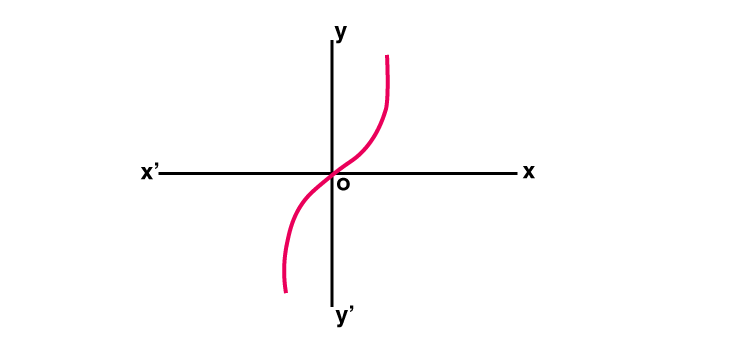
\includegraphics[scale=0.25]{hyperbolicfunction1.png}
    \end{center}
    -    in $f(x) = x^{3} + 1$ the constant 1 is the y intercept
    \newline
    If the form is $kx^{3}$ when $k>0$ it is a increasing function and when $k<0$ it is a decreassing function.
    The point of inflection in the $x^{3}$ function is wear the gradient of the line changes
    \newline
    To find the point of inflexion we can get the equation in the form $f(x) = k(x-b)^{3}+c$ which is the same as $kx^{3}$ however the inflexion point is $(b,c)$
    \newline
    The final way a cubic function can be displayed is of $ f(x) = k(x-a)(x-b)(x-c)$


}
\qs{}{\begin{center} Find inflexion point of the equation $2(x-1)^{3}-16$ \end{center} }
$$=k(x-b)^{3} + c$$
$$POI = (b,c)$$
$$POI=(1,16)$$
\qs{}{\begin{center} Find inflexion point of the equation $(x+2)^{3}+8=0$ \end{center} }
$$=k(x-b)^{3} + c$$
$$POI = (b,c)$$
$$POI = (-2,8)$$
\begin{note} 
    As the form is -b, the b value for POI is negative rather than positive. If the b vlue was negative it the POI b would be positive.
\end{note}

\subsection{Hyperbolic Function(Inverse variation)}
\thm{Hyperbolic Function}{
    A hyperbola occurs in the form of $\frac{k}{x}$ where k is a constant. This equation tells us that when one variable increases the other decreases..
    \newline
    A hyperbola is a discontinuous function meaning there are gaps. There are two asymptotes in a hyperbolic function one on the $x$ and one on the $y$ axis. 
    \begin{center}
        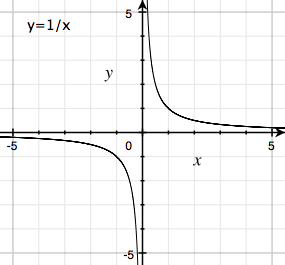
\includegraphics[scale=0.5]{hyperbolafunction1.png}
    \end{center}
    To find the y intercept set x = 0 and solve for y
    \newline
    To find the x asymptote  solve expression on the denominator for x.
    \newline
    To find the y asymptote  substitute the x asymtote into the denominator expression and solve for y
        

}

\qs{}{\begin{center} Find the asymptotes and the Domain and Range of the following function $f(x) = \frac{3}{x-3} \end{center}$ }
$$x-3 \neq 0$$
$$x \neq 3$$
$$y \neq 0$$
\begin{center} y int $\neq\frac{3}{0-3}$\end{center}
\begin{center} y int $\neq-1$\end{center}
\begin{center}
    $\therefore$ x asymptote $= 3$, y asymptote $= 0$, y int $= 0$
\end{center}
\begin{center}   
    Domain:
    \newline
    $(-\infty, 3)\cup(3,\infty) $
    \newline
    Range:
    \newline
    $(-\infty,0)\cup(0,\infty)$
\end{center}
\newpage
\qs{}{\begin{center} Find the x and y asymptotes and the y intercept = for the following function $f(x)= -\frac{1}{2x+4}$   \end{center}}
\begin{center}
    $2x+4 \neq 0$
    \newline
    $2x \neq -4$
    \newline
    $x \neq -2$
    \newline
    x asymp $= -2$
    \newline
    y int $= -\frac{1}{0+4}$
    \newline
    y int $= -\frac{1}{4}$
    \newline
    y asymp $= 0$

\end{center}


\subsection{Linear functions}
\subsubsection{Intersection of Two Lines}
\thm{Intersection of two lines}{
    To find the point where two lines intersect we need to solve the two equations simultaneously
}
\qs{}{\begin{center} Find the intersection points of the equations $4x+2y+2=0$ and $3x+5y-9=0$\end{center}}
$$4x+2y+2=0...1$$
$$3x+5y-9=0...2$$
$$...1 \times 3$$
$$12x+6y+6 = 0...3$$
$$...2 \times 4$$
$$12x+20y-36=0...4$$
$$...4 - ...3$$
$$14y - 42 = 0$$
$$y = 3$$
$$4x+6+2 = 0$$
$$x = -2$$
\begin{center}
    $\therefore$ the intersection point of the two lines is $(-2,3)$
\end{center}

\qs{}{Find the equuation of the line above if it passes through points $(4, -2)$}

$$m = \frac{3+2}{-2-4}$$
$$m = -\frac{5}{6}$$
$$y - 3 = -\frac{5}{6}(x+2)$$
$$y-3 = -\frac{5}{6}x + -\frac{10}{6}$$
$$6y-18 = -5x -10$$
$$5x+6y-8 =0$$
\begin{note}
    Two straight lines have three possible variations with them intersecting at the same point, being parallel or coinciding(infinite solutions)
\end{note}
\subsubsection{Solving Simultaneous equations using the k method}
\thm{K method}{}
    \end{document}